\documentclass[tikz,border=6pt]{standalone}
\usepackage{amsmath}
\usepackage{newtxtext,newtxmath}
\usetikzlibrary{arrows.meta,calc}

\begin{document}
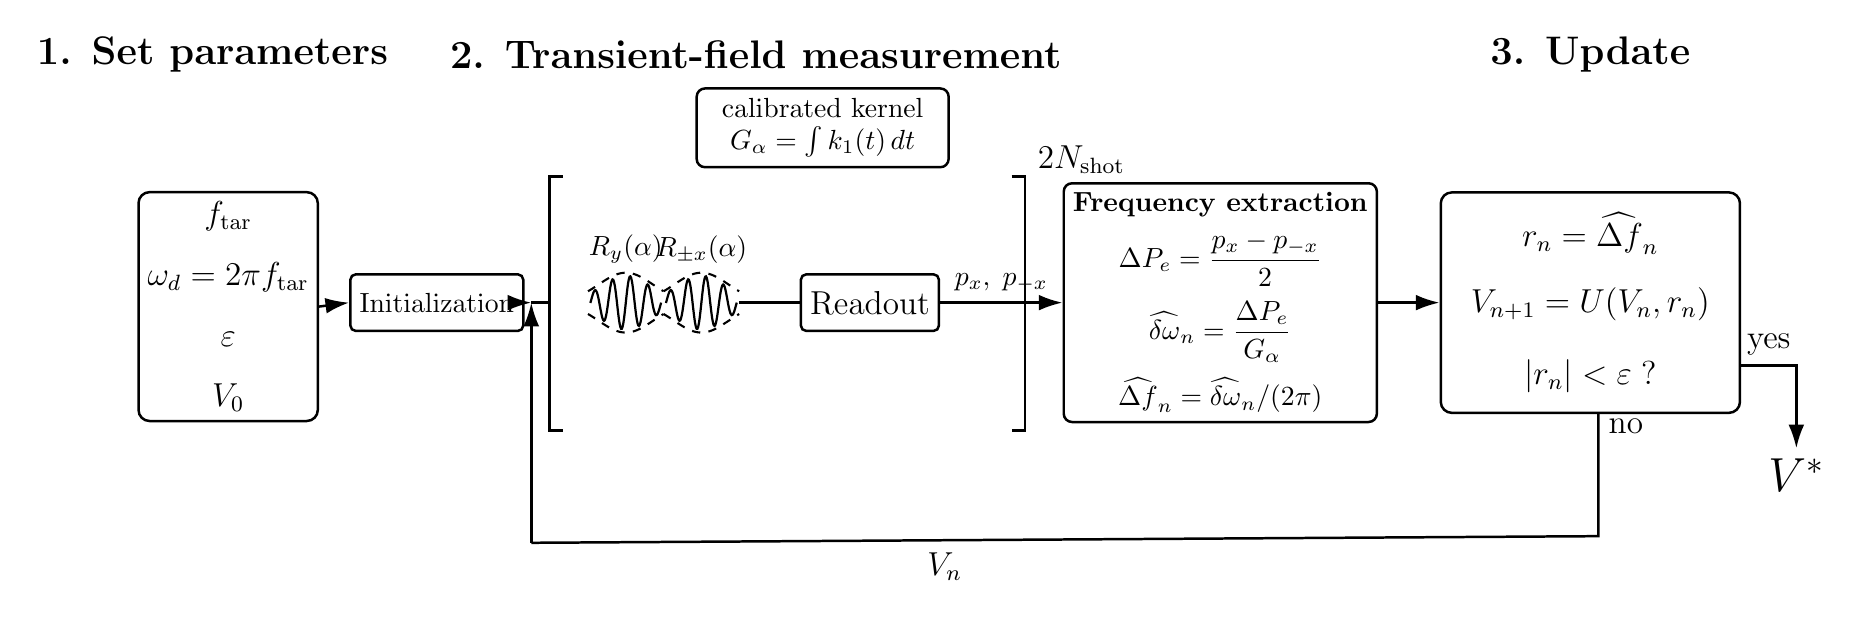
\begin{tikzpicture}[
  x=1cm,
  y=1cm,
  >=Latex,
  font=\large,
  line/.style={draw=black,line width=0.9pt},
  arrow/.style={line,-{Latex[length=3mm,width=2mm]}},
  block/.style={line,rounded corners=2pt,align=center,minimum height=0.72cm},
  setbox/.style={line,rounded corners=4pt,align=center,minimum width=1.7cm,minimum height=2.9cm},
  updatebox/.style={line,rounded corners=4pt,align=center,minimum width=3.8cm,minimum height=2.8cm},
  extractbox/.style={line,rounded corners=3pt,align=center,minimum width=3.9cm,minimum height=1.65cm,font=\normalsize},
  kernelbox/.style={line,rounded corners=3pt,align=center,minimum width=3.2cm,minimum height=1.0cm,font=\normalsize},
  smallblock/.style={block,minimum width=1.3cm},
  pulse/.style={line,line width=0.8pt},
  envelope/.style={line,dashed,line width=0.75pt}
]

% Section headings
\node[font=\bfseries\Large] at (0.3,3.35) {1. Set parameters};
\node[font=\bfseries\Large] at (7.2,3.35) {2. Transient-field measurement};
\node[font=\bfseries\Large] at (17.8,3.35) {3. Update};

% Set parameters
\node[setbox] (set) at (0.5,0.15) {$f_{\mathrm{tar}}$\\[0.28cm]$\omega_d=2\pi f_{\mathrm{tar}}$\\[0.28cm]$\varepsilon$\\[0.28cm]$V_0$};

% Measurement bracket
\draw[line width=1pt]
  (4.75,1.80) -- (4.58,1.80) -- (4.58,-1.42) -- (4.75,-1.42);
\draw[line width=1pt]
  (10.45,1.80) -- (10.62,1.80) -- (10.62,-1.42) -- (10.45,-1.42);
\node[anchor=south west,font=\large] at (10.66,1.72) {$2N_{\mathrm{shot}}$};

% Entry and initialization
\node[smallblock,minimum width=1.45cm,font=\normalsize] (init) at (3.15,0.20) {Initialization};
\draw[arrow] (set.east) -- (init.west);
\draw[arrow] (init.east) -- (4.35,0.20);
\draw[line] (4.35,0.20) -- (4.58,0.20);

% Pulse sequence: Ry - R_{+-x}
\node[font=\normalsize] at (5.55,0.88) {$R_y(\alpha)$};
\begin{scope}[shift={(5.55,0.20)}]
  \draw[pulse,domain=-0.45:0.45,samples=100,smooth]
    plot (\x,{0.34*exp(-5*\x*\x)*sin(deg(28*\x))});
  \draw[envelope,domain=-0.48:0.48,samples=60,smooth]
    plot (\x,{0.38*exp(-4.2*\x*\x)});
  \draw[envelope,domain=-0.48:0.48,samples=60,smooth]
    plot (\x,{-0.38*exp(-4.2*\x*\x)});
\end{scope}

\node[font=\normalsize] at (6.51,0.88) {$R_{\pm x}(\alpha)$};
\begin{scope}[shift={(6.51,0.20)}]
  \draw[pulse,domain=-0.45:0.45,samples=100,smooth]
    plot (\x,{0.34*exp(-5*\x*\x)*sin(deg(28*\x))});
  \draw[envelope,domain=-0.48:0.48,samples=60,smooth]
    plot (\x,{0.38*exp(-4.2*\x*\x)});
  \draw[envelope,domain=-0.48:0.48,samples=60,smooth]
    plot (\x,{-0.38*exp(-4.2*\x*\x)});
\end{scope}

\node[smallblock,minimum width=1.1cm] (readout) at (8.65,0.20) {Readout};
\draw[line] (6.99,0.20) -- (readout.west);

% Pre-calibrated kernel inset
\node[kernelbox] (kernel) at (8.05,2.42)
  {calibrated kernel\\[-0.02cm] $G_\alpha=\int k_1(t)\,dt$};

% Frequency extraction
\node[extractbox] (extract) at (13.1,0.20)
  {\textbf{Frequency extraction}\\[0.16cm]
   $\Delta P_e=\dfrac{p_x-p_{-x}}{2}$\\[0.16cm]
   $\widehat{\delta\omega}_n=\dfrac{\Delta P_e}{G_\alpha}$\\[0.16cm]
   $\widehat{\Delta f}_n=\widehat{\delta\omega}_n/(2\pi)$};
\draw[arrow] (readout.east) -- node[above,font=\normalsize] {$p_x,\;p_{-x}$} (extract.west);

% Update
\node[updatebox] (update) at (17.8,0.20)
  {$r_n=\widehat{\Delta f}_n$\\[0.35cm]
   $V_{n+1}=U(V_n,r_n)$\\[0.42cm]
   $|r_n|<\varepsilon\;?$};
\draw[arrow] (extract.east) -- (update.west);

% Output and feedback
\draw[arrow] ($(update.east)+(0,-0.8)$) -- ++(0.7,0)
  node[midway,above] {yes} -- ++(0,-1.05)
  node[below,font=\LARGE] {$V^\ast$};

\draw[line] ($(update.south)+(0.1,0)$) -- ++(0,-1.55)
  node[right,pos=0.1] {no} -- (4.35,-2.85);
\draw[arrow] (4.35,-2.85) -- (4.35,0.20);
\node[font=\large] at (9.6,-3.15) {$V_n$};

\end{tikzpicture}
\end{document}
